\chapter{Introduzione alle Tecnologie del Linguaggio Naturale}

\section{Prologo}

La prima parte del corso sarà incentrata sulla linguistica computazionale generale, in cui ci si soffermerà sugli aspetti più tradizionali e linguistici\footnote{Libro di riferimento: An Introduction to Natural Language Processing,
Computational Linguistics, and Speech Recognition. La prima e la seconda edizione, perché Jurafsky non riesce a finire il draft della terza :(}. In questa parte verrà anche trattato il parsing. Nella seconda parte si andranno a studiare la semantica lessicale e le ontologie. Infine, nella terza parte del corso si andrà a studiare NLP statistico e distribuzionale.

\begin{figure}[h]
    \centering
    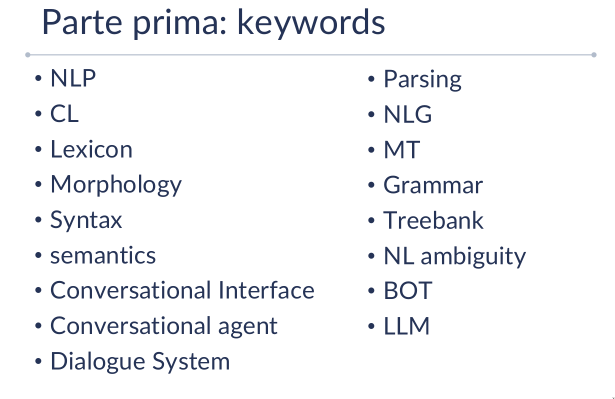
\includegraphics[scale=0.75]{01/key.png}
    \caption{Il giorno prima dell'esame bisogna sapere cosa significano tutte queste parole :3}
\end{figure}

\paragraph{Le 4 ere della linguistica computazionale:}

\begin{enumerate}
  \item 1940 - 1969: primi tentativi. 
  \item 1970 - 1992: formalizzazione. 
  \item 1993 - 2012: apprendimento automatico. 
  \item 2013 - 2018: deep learning.
\end{enumerate}

\nt{Tutto cambiò nel 2018, quando NLP fu il primo successo su larga scala di rete neurale autosupervisionata.}

\begin{figure}[h]
    \centering
    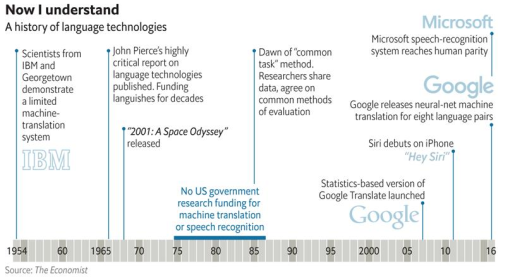
\includegraphics[scale=0.75]{01/timeline.png}
    \caption{Il passato delle tecnologie del linguaggio naturale.}
\end{figure}

\subsection{La Complessità del Linguaggio Naturale}

C'è un legame tra linguaggio umano e intelligenza. Già Turing sosteneva che se si potesse parlare in un certo modo si fosse intelligenti (test di Turing). La differenza tra il linguaggio umano e un linguaggio di programmazione è l'\fancyglitter{ambiguità}: C o Java non sono ambigui.

\paragraph{Il linguaggio umano:}

\begin{itemize}
  \item \fancyglitter{Discretezza} (esistenza di elementi): 
    \begin{itemize}
      \item Api: Ritmo, orientamento, durata. 
      \item Esseri umani: Fonemi, morfemi, parole.
    \end{itemize}
  \item \fancyglitter{Ricorsività}: 
    \begin{itemize}
      \item Scimpanze: Gesti atomici. 
      \item Uomo: Gianni vede Pietro, Maria vuole che Gianni veda Pietro, Paolo crede che Maria voglia che Gianni veda Pietro.
    \end{itemize}
  \item \fancyglitter{Dipendenza dalla struttura}: 
    \begin{itemize}
      \item Non “una parola dietro l'altra” ma c'è una struttura: La ragazza parte, I ragazzi di cui mi ha parlato la ragazza partono. 
    \end{itemize}
  \item \fancyglitter{Località}: 
    \begin{itemize}
      \item Gianni lo ha guardato. 
      \item Gianni ha detto che Pietro lo ha guardato.
    \end{itemize}
\end{itemize}

\paragraph{Intelligenza e linguaggio nel il test di Turing:}

\begin{itemize}
  \item Possono le macchine pensare?
  \item Se riesco a parlare come un essere umano allora penso. 
  \item Gioco dell'imitazione: un giudice deve capire se quello che ha davanti è un uomo oppure un computer.
\end{itemize}

\nt{Ci sono una serie di obiezioni a questo test: teologia, matematica, coscienza, etc.}

\begin{figure}[h]
    \centering
    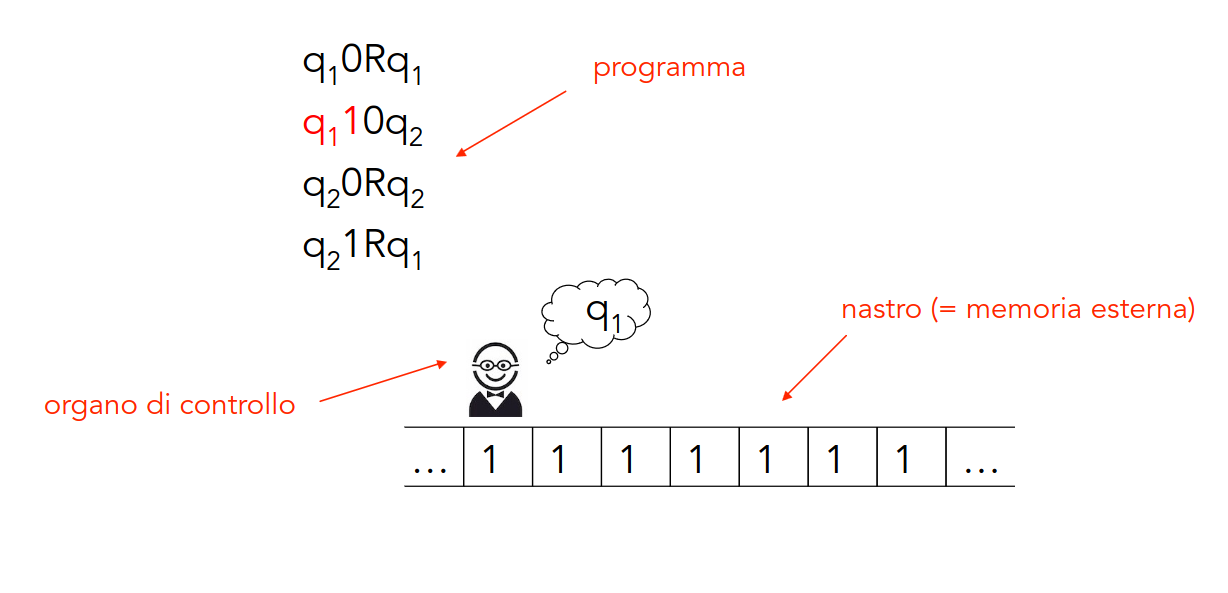
\includegraphics[scale=0.6]{01/Turing.png}
    \caption{Il gioco dell'imitazione.}
\end{figure}

\subsubsection{}

Nel 1966, Weizenbaum crea Eliza. Una macchina in grado di "comprendere" e ingannare gli esseri umani.

\nt{Il punto debole del test di Turing e di Eliza è il giudice: se è coinvolto emotivamente potrebbe far passare un computer per un essere umano\footnote{Blade runner moment}.}

\dfn{Winograd Schema}{
  Evoluzione del Turing test: un test a scelta multipla che utilizza domande con una specifica struttura. In questi test gli esseri umani sono molto bravi a rispondere, i computer no. 
}

\nt{Rimuove il giudizio, quindi tecnicamente più accurato.}

\cor{Captcha}{
  Un test di Turing inverso per capire se l'interloquitore è umano. Non c'è linguaggio, ma riconoscimento cognitivo.
}

\cor{Voight-Kampff Test}{
  Test in Blade runner basato sulle emozioni, evoluzione del test di Turing.
}

\subsection{I Livelli di Conoscenza del Linguaggio}

HAL 9000, in "2001: Odissea nello spazio" mostra un esempio di comunicazione. 

\qs{}{Come fa HAL a rispondere?}

\begin{itemize}
  \item Riconoscimento vocale. 
  \item Comprensione del linguaggio naturale. 
  \item Generazione del linguaggio naturale. 
  \item Sintesi vocale. 
  \item Recupero ed estrazione di informazioni. 
  \item Inferenza.
\end{itemize}

\paragraph{Livelli della conoscenza:}

\begin{enumerate}
  \item Il suono: HAL deve essere in grado di analizzare e produrre
dei segnali audio che contengono le parole: foni e
fonemi. 
\item Le parole: HAL deve essere in grado di riconoscere le singole
parole. 
\item Raggruppare le parole: HAL deve essere in grado di distinguere la struttura
della frase. 
\item Significato: HAL deve conoscere il significato delle singole
parole e deve essere in grado di comporre questi
significati per trovare il significato complessivo
della frase. 
\item Contesto e scopi: HAL deve avere delle conoscenze del mondo che
gli permettono usare il linguaggio in maniera
contestuale: \textit{I’m afraid, I can’t} invece di \textit{I won't}.
\item Conversazione: HAL deve avere deve essere in grado di
conversare, dando delle risposte e facendo delle
domande pertinenti al discorso. 
\end{enumerate}

\paragraph{A ogni livello corrisponde una parte del linguaggio:}

\begin{enumerate}
  \item Fonetica e Fonologia: lo studio del suono della lingua. 
  \item Morfologia: lo studio delle parti significative delle parole. 
  \item Sintassi: lo studio sulla struttura e sulle relazioni tra le parole. 
  \item Semantica: lo studio del significato. 
  \item Pragmatica: lo studio di come il linguaggio è usato per compiere goal. Il passivo serve per mettere in luce/enfatizzare alcune parti della frase. 
  \item Discorso: lo studio delle unità linguistiche rispetto alla singola dichiarazione.
\end{enumerate}

\nt{Jurafsky è un chad nerd.}















